\documentclass[border=4pt,12pt]{standalone}
% House style for redrawn exam diagrams (diagram-v4: 0.4pt lines, filled -latex arrows, fine dashes; stipple and hatching drawn as real dots/lines (no PDF/SVG patterns, so they render in every browser and at any scale); transparent background). Every figure \input's this.
\usepackage{amsmath,amssymb}
\usepackage{txfonts}
\usepackage{pdfrender,xcolor}
% \halo{text}: label on shading. The shading stops just around each letter's outline (a thin knock-out that follows the
% glyphs, like the papers' typesetting), never a box. Owner: "I don't want a box around the text".
\newcommand{\halo}[1]{\leavevmode\rlap{\pdfrender{TextRenderingMode=2,LineWidth=2.2pt,LineJoinStyle=1,StrokeColor=white,FillColor=white}#1}#1}
\usepackage{tikz,pgfplots}
\pgfplotsset{compat=1.18}
\usetikzlibrary{arrows.meta,calc,angles,quotes,patterns,patterns.meta,intersections,positioning,decorations.markings,shapes.geometric}
% Stipple and hatching are drawn as actual dots / lines clipped to the region (path picture), NOT as pattern fills:
% SVG <pattern> fills vanish or blur when browsers scale the image, so the owner could not see the shading.
% Each dot is a 0.72pt square (keeps SVGs small; reads as a dot at print size). Dots sit on one global staggered grid, so neighbouring regions line up.
\makeatletter
\newdimen\ex@x \newdimen\ex@y \newdimen\ex@xa \newdimen\ex@ya \newdimen\ex@xb \newdimen\ex@yb \newcount\ex@row
\def\exam@stipplecolor{black!75}\def\exam@dotr{0.42pt}\def\exam@dotgap{2.5}
\def\ex@rowdots{\ifdim\ex@x<\ex@xb \pgfpathrectangle{\pgfqpoint{\dimexpr\ex@x-0.36pt\relax}{\dimexpr\ex@y-0.36pt\relax}}{\pgfqpoint{0.72pt}{0.72pt}}\advance\ex@x by \exam@dotgap pt\relax\expandafter\ex@rowdots\fi}
\def\exam@stipple{%
  \pgftransformreset% dots are sized in real points even inside scaled pictures
  \pgfpointanchor{path picture bounding box}{south west}\ex@xa=\pgf@x \ex@ya=\pgf@y
  \pgfpointanchor{path picture bounding box}{north east}\ex@xb=\pgf@x \ex@yb=\pgf@y
  \pgfsetfillcolor{\exam@stipplecolor}\pgfmathsetmacro\ex@h{\exam@dotgap/2}%
  \pgfmathtruncatemacro\ex@r{floor(\ex@ya/\ex@h)-1}\ex@row=\ex@r\relax
  \ex@y=\ex@r\dimexpr\ex@h pt\relax
  \loop\ifdim\ex@y<\ex@yb
    \pgfmathtruncatemacro\ex@c{floor(\ex@xa/\exam@dotgap)-1}\ex@x=\ex@c\dimexpr\exam@dotgap pt\relax
    \ifodd\ex@row \advance\ex@x by \ex@h pt\fi
    \ex@rowdots
    \advance\ex@y by \ex@h pt \advance\ex@row by 1
    \ifnum\numexpr\ex@row-(\ex@row/4)*4\relax=0 \pgfusepath{fill}\fi% flush every 4 rows: bounded TeX memory, few clip copies in the SVG
  \repeat\pgfusepath{fill}}
\newdimen\ex@d
\def\exam@hatch#1{% #1 = 1 for /, -1 for \ ; lines 45 degrees, 3pt apart
  \pgftransformreset
  \pgfpointanchor{path picture bounding box}{south west}\ex@xa=\pgf@x \ex@ya=\pgf@y
  \pgfpointanchor{path picture bounding box}{north east}\ex@xb=\pgf@x \ex@yb=\pgf@y
  \ex@d=\dimexpr\ex@yb-\ex@ya\relax \ex@x=\dimexpr\ex@xa-\ex@d\relax
  \loop\ifdim\ex@x<\ex@xb
    \ifnum#1>0 \pgfpathmoveto{\pgfqpoint{\ex@x}{\ex@ya}}\pgfpathlineto{\pgfqpoint{\dimexpr\ex@x+\ex@d\relax}{\ex@yb}}%
    \else \pgfpathmoveto{\pgfqpoint{\ex@x}{\ex@yb}}\pgfpathlineto{\pgfqpoint{\dimexpr\ex@x+\ex@d\relax}{\ex@ya}}\fi
    \advance\ex@x by 4.24pt
  \repeat
  \pgfsetlinewidth{0.4pt}\pgfsetstrokecolor{black}\pgfusepath{stroke}}
\def\examstipple{\exam@stipple}\def\examhatch{\exam@hatch}\def\examsetstipplecolor#1{\def\exam@stipplecolor{#1}}\def\examsetdotgap#1{\def\exam@dotgap{#1}}
\makeatother
% (legacy pattern kept for old files)
% staggered stipple like the NESA papers' dotted shading
\pgfdeclarepatternformonly{exam stipple}{\pgfpointorigin}{\pgfqpoint{2.2pt}{2.2pt}}{\pgfqpoint{2.2pt}{2.2pt}}{%
  \pgfpathcircle{\pgfqpoint{0.55pt}{0.55pt}}{0.42pt}\pgfpathcircle{\pgfqpoint{1.65pt}{1.65pt}}{0.42pt}\pgfusepath{fill}}
\tikzset{
  every picture/.style={line width=0.6pt, >={Latex[length=2mm,width=1.3mm]}},
  curve/.style={line width=0.6pt},
  open arrow/.style={-{Latex[length=2mm,width=1.3mm]}},  % owner: filled -latex heads everywhere, no open chevrons
  aux/.style={dash pattern=on 2pt off 1.5pt, line width=0.6pt},
  shade/.code={\def\exA{#1}\def\exB{none}\ifx\exA\exB\else\pgfkeysalso{fill=black!18}\fi},
  shade/.default=on,
  shade dots/.style={fill=none, path picture={\examstipple}},
  stipple color/.code={\examsetstipplecolor{#1}},
  stipple gap/.code={\examsetdotgap{#1}},
  shade dense dots/.style={fill=none, stipple gap=1.6, path picture={\examstipple}},
  shade hatch/.style={fill=none, path picture={\examhatch{1}}},
  shade hatch reverse/.style={fill=none, path picture={\examhatch{-1}}},
  shade solid/.style={fill=black},
  pt/.style={circle, fill, inner sep=1.1pt},
  open pt/.style={circle, draw, fill=white, inner sep=1.1pt},
}
\pgfplotsset{
  exam axes/.style={axis lines=middle, axis line style={->}, xlabel={$x$}, ylabel={$y$},
    xlabel style={anchor=west}, ylabel style={anchor=south}, tick label style={font=\small},
    every axis plot/.append style={line width=0.6pt, black}, samples=200, clip=false,
    enlargelimits=false, axis on top},
}

\begin{document}
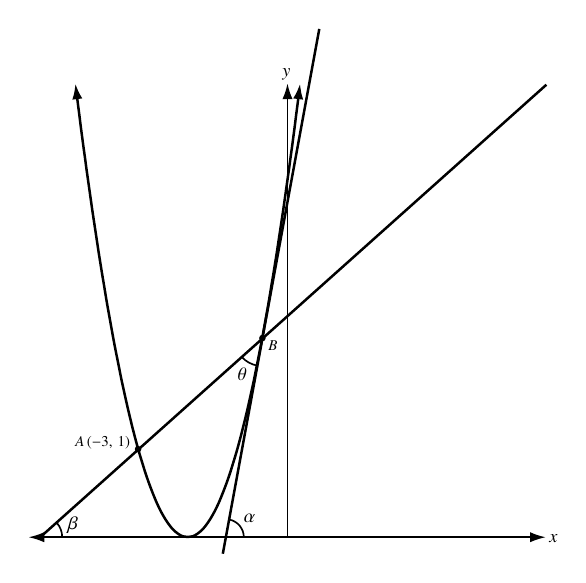
\begin{tikzpicture}[x=0.0127cm,y=-0.0127cm,font=\fontsize{5.4}{6.5}\selectfont]
\draw[<->] (74.4,518.5) -- (591.9,518.5);
\draw[->] (333.5,518.5) -- (333.5,64.5);
\node[anchor=base,inner sep=0,font=\fontsize{6.6}{8}\selectfont] at (599,524) {$x$};
\node[anchor=base,inner sep=0,font=\fontsize{6.6}{8}\selectfont] at (332.5,58) {$y$};
\draw[<->, line width=0.9pt] plot[smooth] coordinates {(121.3,64.5) (122.6,75.1) (123.9,85.7) (125.3,96.4) (126.6,107.0) (128.0,117.6) (129.4,128.2) (130.9,138.9) (132.3,149.5) (133.8,160.1) (135.3,170.7) (136.8,181.3) (138.3,191.9) (139.9,202.5) (141.5,213.1) (143.1,223.7) (144.7,234.3) (146.4,244.9) (148.1,255.5) (149.9,266.1) (151.6,276.6) (153.4,287.2) (155.3,297.7) (157.2,308.3) (159.1,318.8) (161.1,329.4) (163.2,339.9) (165.3,350.4) (167.4,360.9) (169.7,371.4) (172.0,381.8) (174.4,392.3) (176.9,402.7) (179.5,413.1) (182.2,423.4) (185.1,433.8) (188.2,444.0) (191.4,454.3) (194.9,464.4) (198.7,474.4) (202.8,484.3) (207.5,493.9) (213.0,503.1) (219.7,511.5) (228.5,517.5) (238.9,517.5) (247.7,511.5) (254.4,503.1) (259.9,493.9) (264.6,484.3) (268.7,474.4) (272.5,464.4) (276.0,454.3) (279.2,444.0) (282.3,433.8) (285.2,423.4) (287.9,413.1) (290.5,402.7) (293.0,392.3) (295.4,381.8) (297.7,371.4) (300.0,360.9) (302.1,350.4) (304.2,339.9) (306.3,329.4) (308.3,318.8) (310.2,308.3) (312.1,297.7) (314.0,287.2) (315.8,276.6) (317.5,266.1) (319.3,255.5) (321.0,244.9) (322.7,234.3) (324.3,223.7) (325.9,213.1) (327.5,202.5) (329.1,191.9) (330.6,181.3) (332.1,170.7) (333.6,160.1) (335.1,149.5) (336.5,138.9) (338.0,128.2) (339.4,117.6) (340.8,107.0) (342.1,96.4) (343.5,85.7) (344.8,75.1) (346.1,64.5)};
\draw[line width=0.9pt] (86.1,518.5) -- (592.5,65.8);
\draw[line width=0.9pt] (365.3,10.0) -- (268.8,535.0);
\fill (184.0,430.4) circle[radius=3.3];
\fill (308.4,319.3) circle[radius=3.3];
\node[anchor=base,inner sep=0] at (318.5,331.6) {$B$};
\node[anchor=base east,inner sep=0] at (176.8,427.5) {$A\,(-3,\,1)$};
\draw (308.4,319.3) ++(100.4:28) arc[start angle=100.4,end angle=138.3,radius=28];
\node[font=\fontsize{7}{8}\selectfont] at (287.9,355.9) {$\theta$};
\draw (271.8,518.5) ++(0:18) arc[start angle=0,end angle=-79.6,radius=18];
\node[font=\fontsize{7}{8}\selectfont] at (295.5,500.0) {$\alpha$};
\draw (86.1,518.5) ++(0:22) arc[start angle=0,end angle=-41.8,radius=22];
\node[font=\fontsize{7}{8}\selectfont] at (119.0,506.5) {$\beta$};
\end{tikzpicture}
\end{document}
